% Shared standalone design for the editable figure reconstructions.
\documentclass[tikz,border=5pt,10pt]{standalone}
\usepackage[T1]{fontenc}
\usepackage[utf8]{inputenc}
\usepackage{newpxtext,newpxmath}
\usepackage[scaled=.94]{sourcesanspro}
\usepackage{pgfplots}
\pgfplotsset{compat=1.18}
\usetikzlibrary{arrows.meta,calc,positioning,decorations.pathreplacing,
  decorations.markings,patterns,matrix,shapes.geometric,fit,backgrounds,
  intersections,angles,quotes}
\definecolor{ink}{HTML}{203746}
\definecolor{accent}{HTML}{146C78}
\definecolor{muted}{HTML}{667780}
\definecolor{signalred}{HTML}{B94B44}
\color{ink}
\tikzset{>=Latex,line width=.8pt,
  every node/.style={font=\small},
  axis/.style={->,draw=muted,line width=.5pt},
  guide/.style={draw=muted,dashed,line width=.45pt},
  curve/.style={draw=accent,line width=1pt},
  marker/.style={circle,fill=accent,inner sep=1.5pt},
  labelbox/.style={fill=white,inner sep=2pt}}

\begin{document}
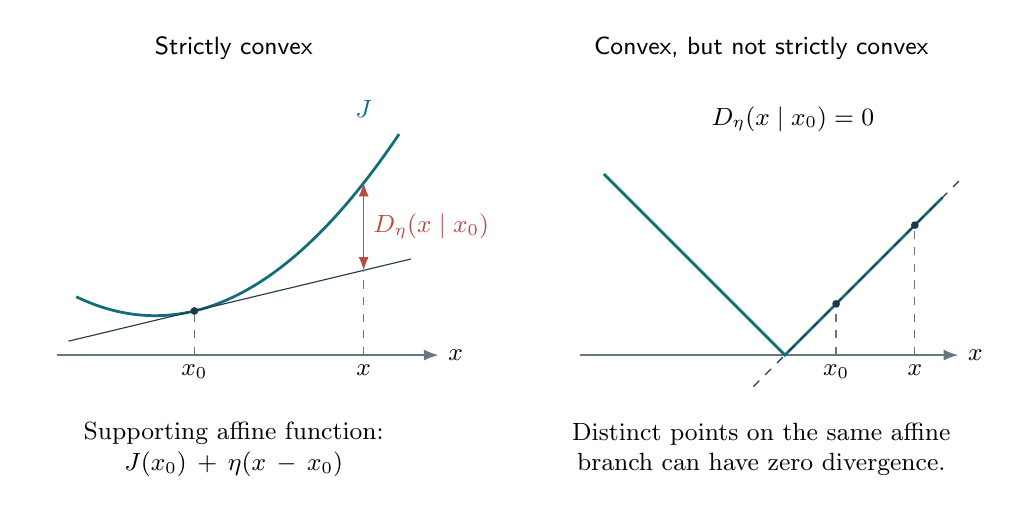
\begin{tikzpicture}
\node[font=\small\sffamily]at(2,3.9){Strictly convex};
\draw[axis](-.25,0)--(4.6,0)node[right]{$x$};
\draw[curve]plot[domain=0:4.1,samples=70](\x,{.24*(\x-1)^2+.5});
\draw[ink](-.1,.176)--(4.25,1.22);
\draw[guide](1.5,0)node[below]{$x_0$}--(1.5,.56);
\draw[guide](3.65,0)node[below]{$x$}--(3.65,1.076);
\fill[ink](1.5,.56)circle(1.4pt);
\draw[<->,signalred](3.65,1.076)--(3.65,2.1854)node[midway,right]{$D_\eta(x\mid x_0)$};
\node[accent]at(3.65,3.12){$J$};
\node[align=center,text width=5cm]at(2,-1.2){Supporting affine function:\\$J(x_0)+\eta(x-x_0)$};
\begin{scope}[shift={(7.0,0)}]
\node[font=\small\sffamily]at(1.7,3.9){Convex, but not strictly convex};
\draw[axis](-.6,0)--(4.2,0)node[right]{$x$};
\draw[curve](-.3,2.3)--(2,0)--(4,2);
\draw[ink,dashed](1.6,-.4)--(4.25,2.25);
\draw[guide](2.65,0)node[below]{$x_0$}--(2.65,.65);\fill[ink](2.65,.65)circle(1.4pt);
\draw[guide](3.65,0)node[below]{$x$}--(3.65,1.65);\fill[ink](3.65,1.65)circle(1.4pt);
\node at(2.1,3){$D_\eta(x\mid x_0)=0$};
\node[align=center,text width=4.9cm]at(1.7,-1.2){Distinct points on the same affine branch can have zero divergence.};
\end{scope}
\end{tikzpicture}
\end{document}
